\chapter{Versuch 3: Leistungsaufnahme eines Widerstand}

\section{Einleitung}
Das Ziel dieses Versuchs besteht darin, die elektrische Leistung zu bestimmen,
die bei Stromdurchfluss durch einen Widerstand R auftritt. Hierfür werden zwei 
unterschiedliche Methoden verwendet. Zum einen wird die Leistung mittels 
direkter Strommessung bestimmt. Zum anderen wird die elektrische Leistung durch
indirekte Strommessung, d.h. über die Spannungsmessung bestimmt. Anschließend 
sollen die Ergebnisse nach Fehlern untersucht und vergliechen werden.

\section{Benötigte Geräte}
Zur Durchführung des Versuchs werden folgende Geräte und Material benötigt:

\begin{tabular}[h]{c|c}
	Widerstand, zwei Stück & 1 k$\Omega$ \textpm 5\% \\
    \hline
    Digital-Multimeter & Fluke TRUE RNS MULTIMETER\\
    \hline
    Steckbrett & \\
    \hline
    Netzgerät & Tenma 72-10495 Digital Control DC Power Supply
    \label{tab:Versuch 3: Geräte}
\end{tabular}

\section{Durchführung}
\subsection{Ausgemessung der Widerstände}
Um die Genauigkeit zu erhöhen, werden die zwei Widerstände R\textsubscript{1}
und R\textsubscript{2} ausgemessen. Widerstand R\textsubscript{1} hat den 
Wert 0,996 k$\Omega$ und Widerstand R\textsubscript{2} hat den Wert 0,985 
k$\Omega$. Somit liegen die Widerstände innerhalb des von dem Hersteller
angegebenen Toleranzbereiches \textpm 5\%. 

\subsection{Direkte Strommessung}
Es wird eine Schaltung aufgebaut, um die Leistung zu bestimmen. Dafür werden
Netzgerät, Widerstand R\textsubscript{1} und Strommessgerät (DMM) in Reihe
geschaltet. Schaltskizze sieht folgendermaßen aus:

\begin{figure}[H]
	\centering
	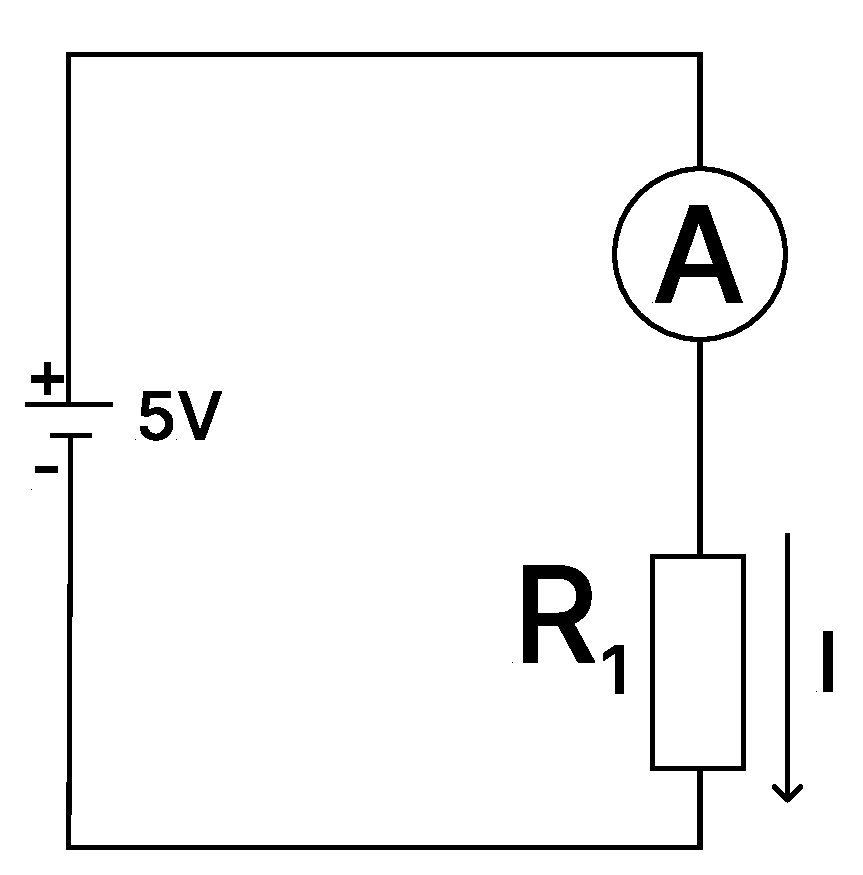
\includegraphics[height=6cm]{images/Versuch3/Versuch3_1_Schaltskizze.pdf} 
	\caption{Schaltungsskizze}
	\label{fig: Schaltungsskizze Versuch 3}
\end{figure}

Mit Hilfe des DMMs wird der Strom gemessen. Dieser beträgt 5.01 mA. Mit der
Formel $P = I^{2}R$ wird die Leistung bestimmt:
$P=(5,01 mA)^{2}\cdot 0,996 k\Omega = 0,02499 W = 24,99mW$.

\subsubsection{Fehlerrechnung}
Fehler durch \textbf{Widerstandsmessung} mit Fluke DMM (Daten aus dem Datenblatt des Fluke DMMs):\\
Bereich 6k$\Omega$, Auflösung 0,001k$\Omega$, Genauigkeit $\pm$(0,02\% + 1 LSD \footnote{Least Significant Digit})\\
Absoluter Fehler: $\Delta R_1 = \pm (0,02\% \cdot R_1 + 1 LSD) = \pm 1,1992 \Omega$\\
Relativer Fehler: $\Delta R_1 = \frac{\Delta R}{R_1} = \frac{1,1992 \Omega}{996 \Omega} = 0,1204\%$\par


Fehler durch \textbf{Strommessung} mit Fluke DMM (Daten aus dem Datenblatt des Fluke DMMs):\\
Bereich 6000$\mu$A, Auflösung 1$\mu$A, Genauigkeit $\pm$(0,2\% + 2 LSD)\\
Absoluter Fehler: $\Delta I = \pm (0,2\% \cdot I + 2 LSD) = \pm 12,02 \mu A$\\
Relativer Fehler: $\Delta I = \frac{\Delta I}{I} = \frac{12,02 \mu A}{5,01 mA} = 0,2399\%$\\

\subsubsection{Maximaler Gesamtfehler}
$\Delta P = 2 \cdot I \cdot R_1 \cdot \Delta I + I^2 \cdot \Delta R_1 = 
2 \cdot I^2 \cdot R_1 \cdot \frac{\Delta I}{I} + I^2 \cdot R_1 \cdot \frac{\Delta R_1}{R_1} =
2 \cdot P \cdot \frac{\Delta I}{I} + P \cdot \frac{\Delta R_1}{R_1} = \\
2 \cdot 24,99 mW \cdot 0,2399\% + 24,99 mW \cdot 0,1204\% = 0,1499 mW $

$\frac{\Delta P}{P} = 2 \cdot \frac{\Delta I}{I} + \frac{\Delta R_1}{R_1} =
2 \cdot 0,2399\% + 0,1204\% = 0,6002\%$

\subsubsection{Wahrscheinlicher Felher}
$ \Delta P = \sqrt{(2 \cdot P \cdot \frac{\Delta I}{I})^2 + (P \cdot \frac{\Delta R_1}{R})^2} =
\sqrt{(2 \cdot 24,99 mW \cdot 0,2399\%)^2 + (24,99 mW \cdot 0,1204\%)^2} = 0,11606mW$

$\frac{\Delta P}{P} = \sqrt{(2 \cdot \frac{\Delta I}{I})^2 + (\frac{\Delta R_1}{R})^2} =
\sqrt{(2 \cdot 0,2399\%)^2 + (0,1204\%)^2} = 0,4946\%$



\subsection{Indirekte Strommessung}
Jetzt soll die elektrische Leistung mit der Methode der indirekten Strommessung
bestimmt werden. Dafür werden der zweite Widerstand, sowie der Spannungsmessgerät
(DMM) in die Schaltung eingebaut. Als R\textsubscript{V} dient der
zweite Widerstand. Die Schaltskizze sieht folgendermaßen aus:

\begin{figure}[H]
	\centering
	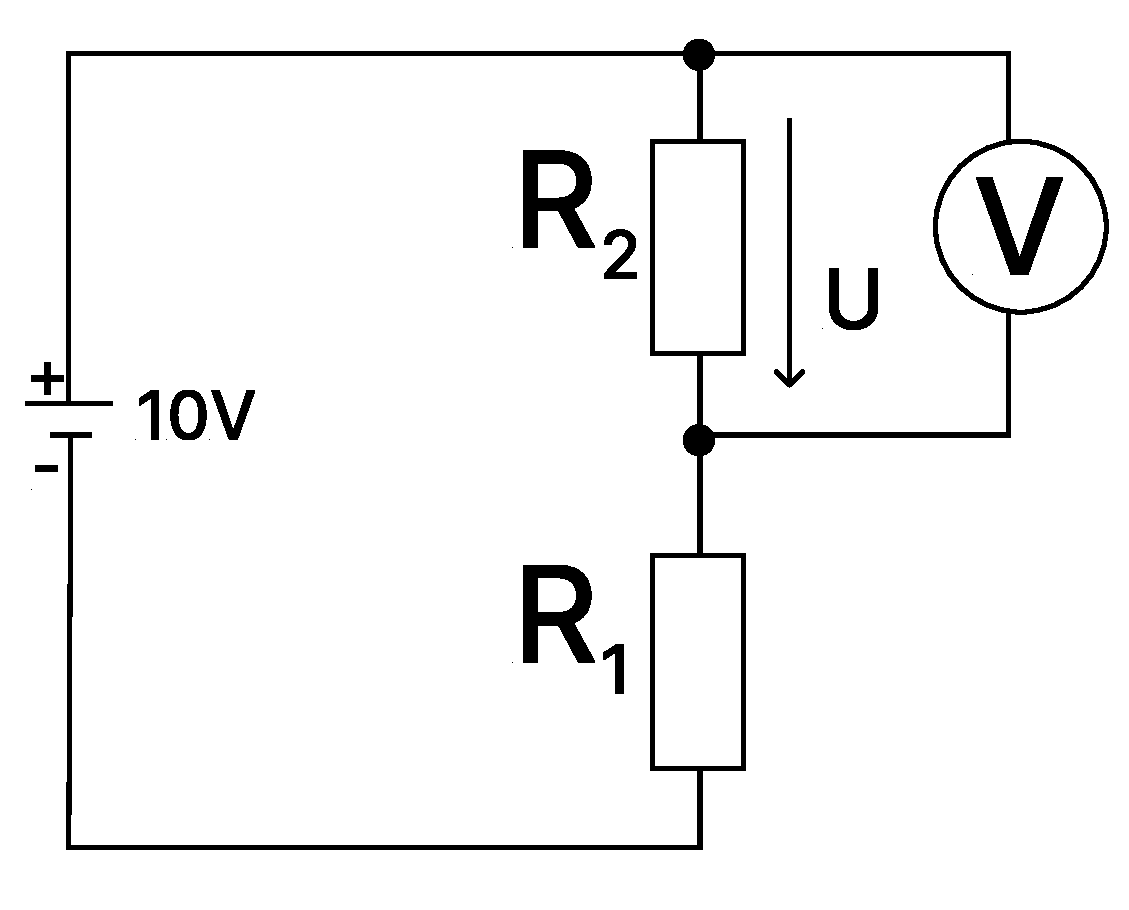
\includegraphics[height=6cm]{images/Versuch3/Versuch3_2_Schaltskizze.pdf} 
	\caption{Schaltungsskizze}
	\label{fig: Schaltungsskizze Versuch 3_2}
\end{figure}

Mit Hilfe des DMMs wird die Spannung gemessen. Diese beträgt 4,964 V. Mit der
Formel $P = (\frac{U}{R\textsubscript{V}})^{2}R$ wird die Leistung bestimmt: 
\[P = (\frac{4,954 V}{0,985 k\Omega})^{2}\cdot 0,996k\Omega = 0,02519 W = 25,19 mW\]

\subsubsection{Fehlerrechnung}
Fehler durch \textbf{Widerstandsmessung} mit Fluke DMM (Daten aus dem Datenblatt des Fluke DMMs):\\
Bereich 6k$\Omega$, Auflösung 0,001k$\Omega$, Genauigkeit $\pm$(0,02\% + 1 LSD)\\
Absoluter Fehler: $\Delta R_1 = \pm (0,02\% \cdot R_1 + 1 LSD) = \pm 1,1992 \Omega$\\
Relativer Fehler: $\Delta R_1 = \frac{\Delta R}{R_1} = \frac{1,1992 \Omega}{996 \Omega} = 0,1204\%$\par

Für R\textsubscript{V} = R\textsubscript{2} gilt analog:
Bereich 6k$\Omega$, Auflösung 0,001k$\Omega$, Genauigkeit $\pm$(0,02\% + 1 LSD)\\
Absoluter Fehler: $\Delta R_2 = \pm (0,02\% \cdot R_2 + 1 LSD) = \pm 1,197\Omega$\\
Relativer Fehler: $\Delta R_2 = \frac{\Delta R}{R_2} = \frac{1,197 \Omega}{985 \Omega} = 0,1215\%$\par

Fehler durch \textbf{Spannungsmessung} mit Fluke DMM (Daten aus dem Datenblatt des Fluke DMMs):\\
Bereich 6V, Auflösung 0,001V, Genauigkeit $\pm$(0,05\% + 1 LSD)\\
Absoluter Fehler: $\Delta U = \pm (0,05\% \cdot U + 1 LSD) = \pm 3,482 mV$\\
Relativer Fehler: $\Delta U = \frac{\Delta U}{U} = \frac{3,482 mV}{4,964 V} = 0,07014\%$\\

\subsubsection{Maximaler Gesamtfehler}
\begin{flalign*}
    |\Delta P| & = |(\frac{U}{R_V})^2| \cdot \Delta R_1 + \abs{-2 \cdot \frac{U^2 \cdot R_1}{R_V^3}} \cdot \Delta R_V + |2 \cdot \frac{U \cdot R_1 }{R_V^2}| \cdot \Delta U \\
    & =\frac{U^2}{R_V^2} \cdot R_1 \cdot (2 \cdot \frac{\Delta R_V}{R_V} + 2 \cdot \frac{\Delta U}{U} + \frac{\Delta R_1}{R_1})
    = P \cdot (2 \cdot \frac{\Delta R_V}{R_V} + 2 \cdot \frac{\Delta U}{U} + \frac{\Delta R_1}{R_1}) \\
    & = 25,19 mW \cdot (2 \cdot 0,1215\% + 2 \cdot 0,07014\% + 0,1204\%)  = 0,1268 mW
\end{flalign*}

\begin{flalign*}
    & \frac{\Delta P}{P} = \frac{0,1268 mW}{25,19 mW} = 0,5033\%
\end{flalign*}

\subsubsection{Wahrscheinlicher Felher}
\begin{flalign*}
    \abs{P} & = P \cdot \sqrt{(2 \cdot \frac{\Delta R_V}{R_V})^2 + (2 \cdot \frac{\Delta U}{U})^2 + (\frac{\Delta R_1}{R_1})^2} \\
    & = 25,19 mW \cdot \sqrt{(2 \cdot 0,1215\%)^2 + (2 \cdot 0,07014\%)^2 + (0,1204\%)^2} = 0,07691 mW
\end{flalign*}

\begin{flalign*}
    & \frac{\Delta P}{P} = \frac{0,07691 mW}{25,19 mW} = 0,3053\%
\end{flalign*}

\subsection{Vergleich der Ergebnisse}



\begin{tabular}[h]{c|c|c}
    & Direkte Strommessung & Indirekte Strommessung \\
    \hline
    Leistung & 24,99 mW & 25,19 mW \\
    \hline
    Maximaler Fehler & 0,6002\% & \cellcolor{green!50}0,5033\% \\
    \hline
    Wahrscheinlicher relativer Fehler & 0,4946\% & \cellcolor{green!50}0,3053\% 
    \label{tab:Versuch 3: Ergebnisse}
\end{tabular}


Die Übersicht zeigt, dass die indirekte Strommessung zu einem genaueren Ergebnis
führt. Dies liegt daran, dass die Fehler der Spannungs- und Widerstandsmessung
geringer sind, als die Fehler der Strommessung.
